\subsection {Possibilities}
  The library consists of two basic functional blocks: The connectivity
  module (librexio) and user interface toolkit (librexiotk). The first
  provides unified interface to screen, while second provides
  extensive set of extensible
  utility classes representing some specific interface
  functionality. Figure below represents typical layout of these items:
  \index{layout}

  \begin{figure}[H]
  \begin{center}
  \leavevmode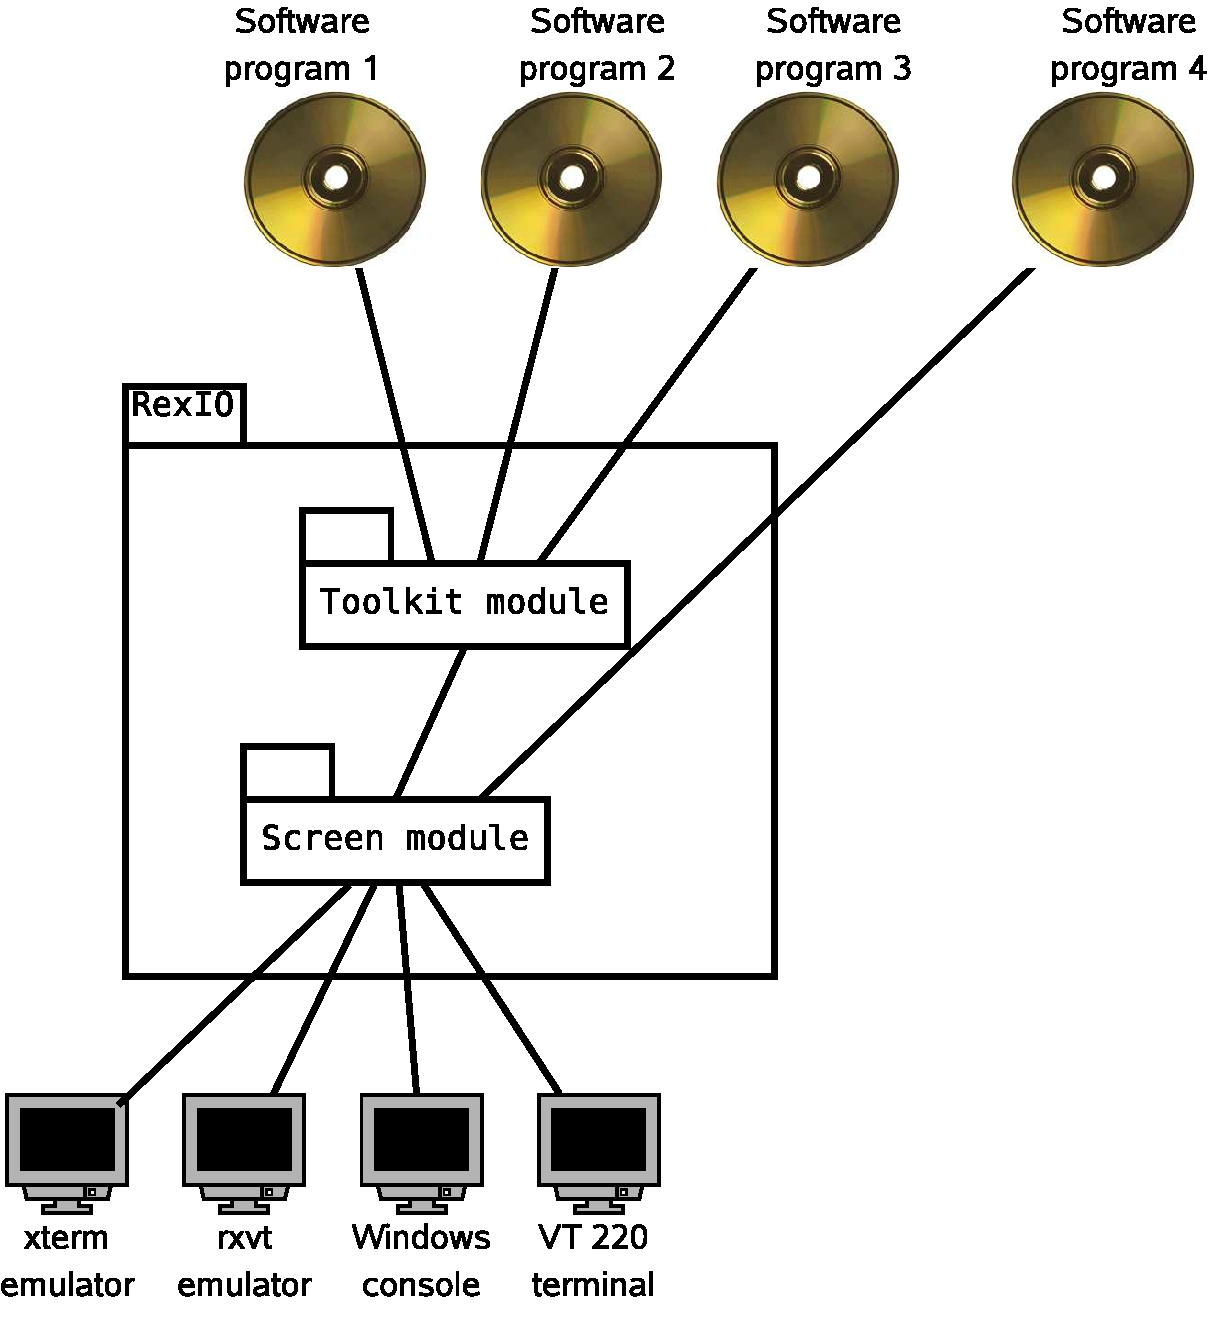
\includegraphics[width=200pt]{graphics/PurposeOfLibrary}
  \end{center}
  \end{figure}

  As you can see, library aims to provide interface to many different
  terminal types, and serve as many software applications as possible.


  Thanks to being object oriented and thread safe, library may allow
  single instance of software program communicate with many clients
  and provide them user interface:

  \begin{figure}[H]
  \begin{center}
  \leavevmode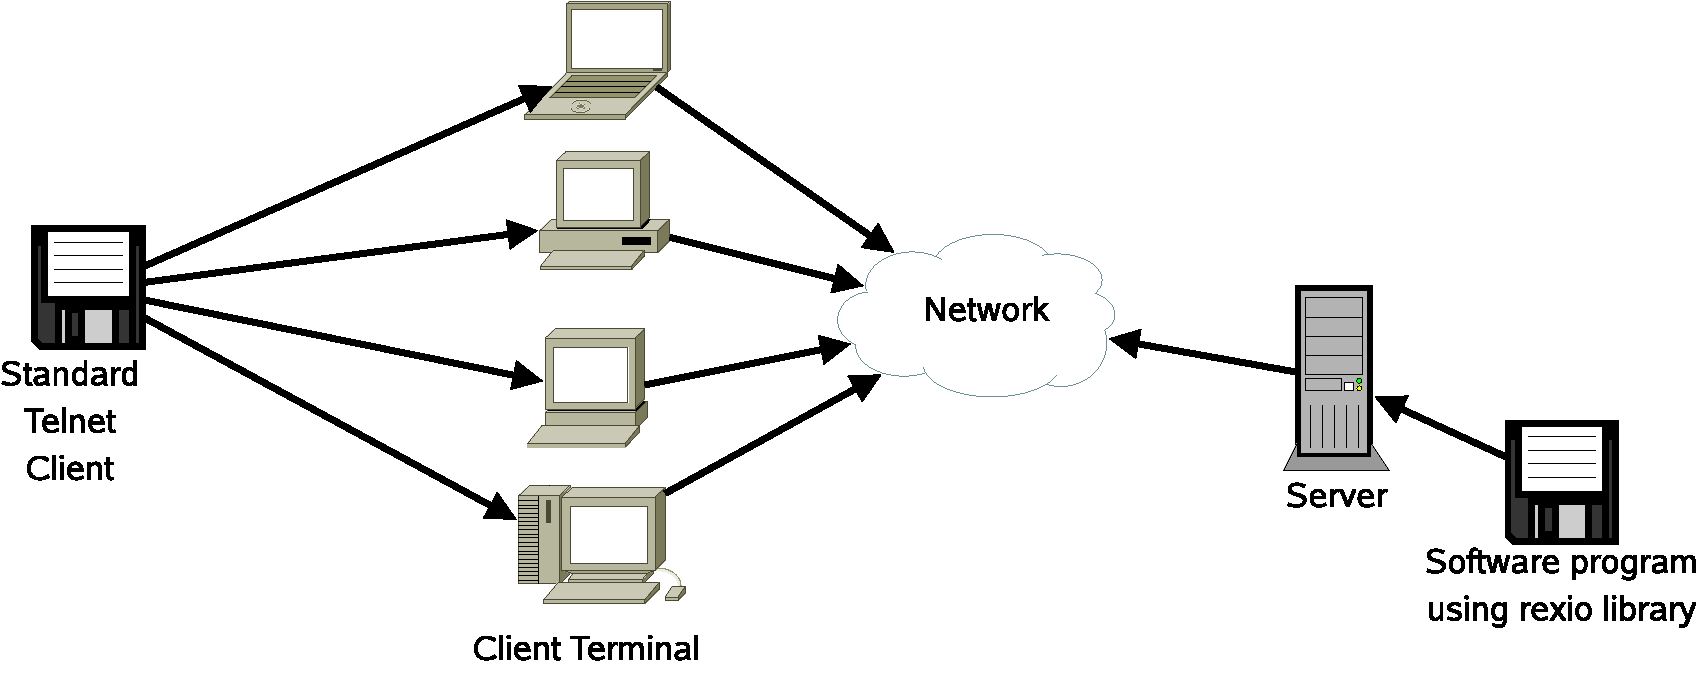
\includegraphics[width=350pt]{graphics/IdeaOfMUD}
  \end{center}
  \end{figure}
  \index{MUD}

  This gives an amazing possibility to create multi user business
  software, collaborative text editors, and also  MMO roleplaying games
  combining availability of traditional MUD's with easy user interface
  of rogue like games. 

\subsection{Internal layout}
  Layout of functional blocks in screen module is as follows:
  \index{subsystems}
  
  \begin{figure}[H]
  \begin{center}
  \leavevmode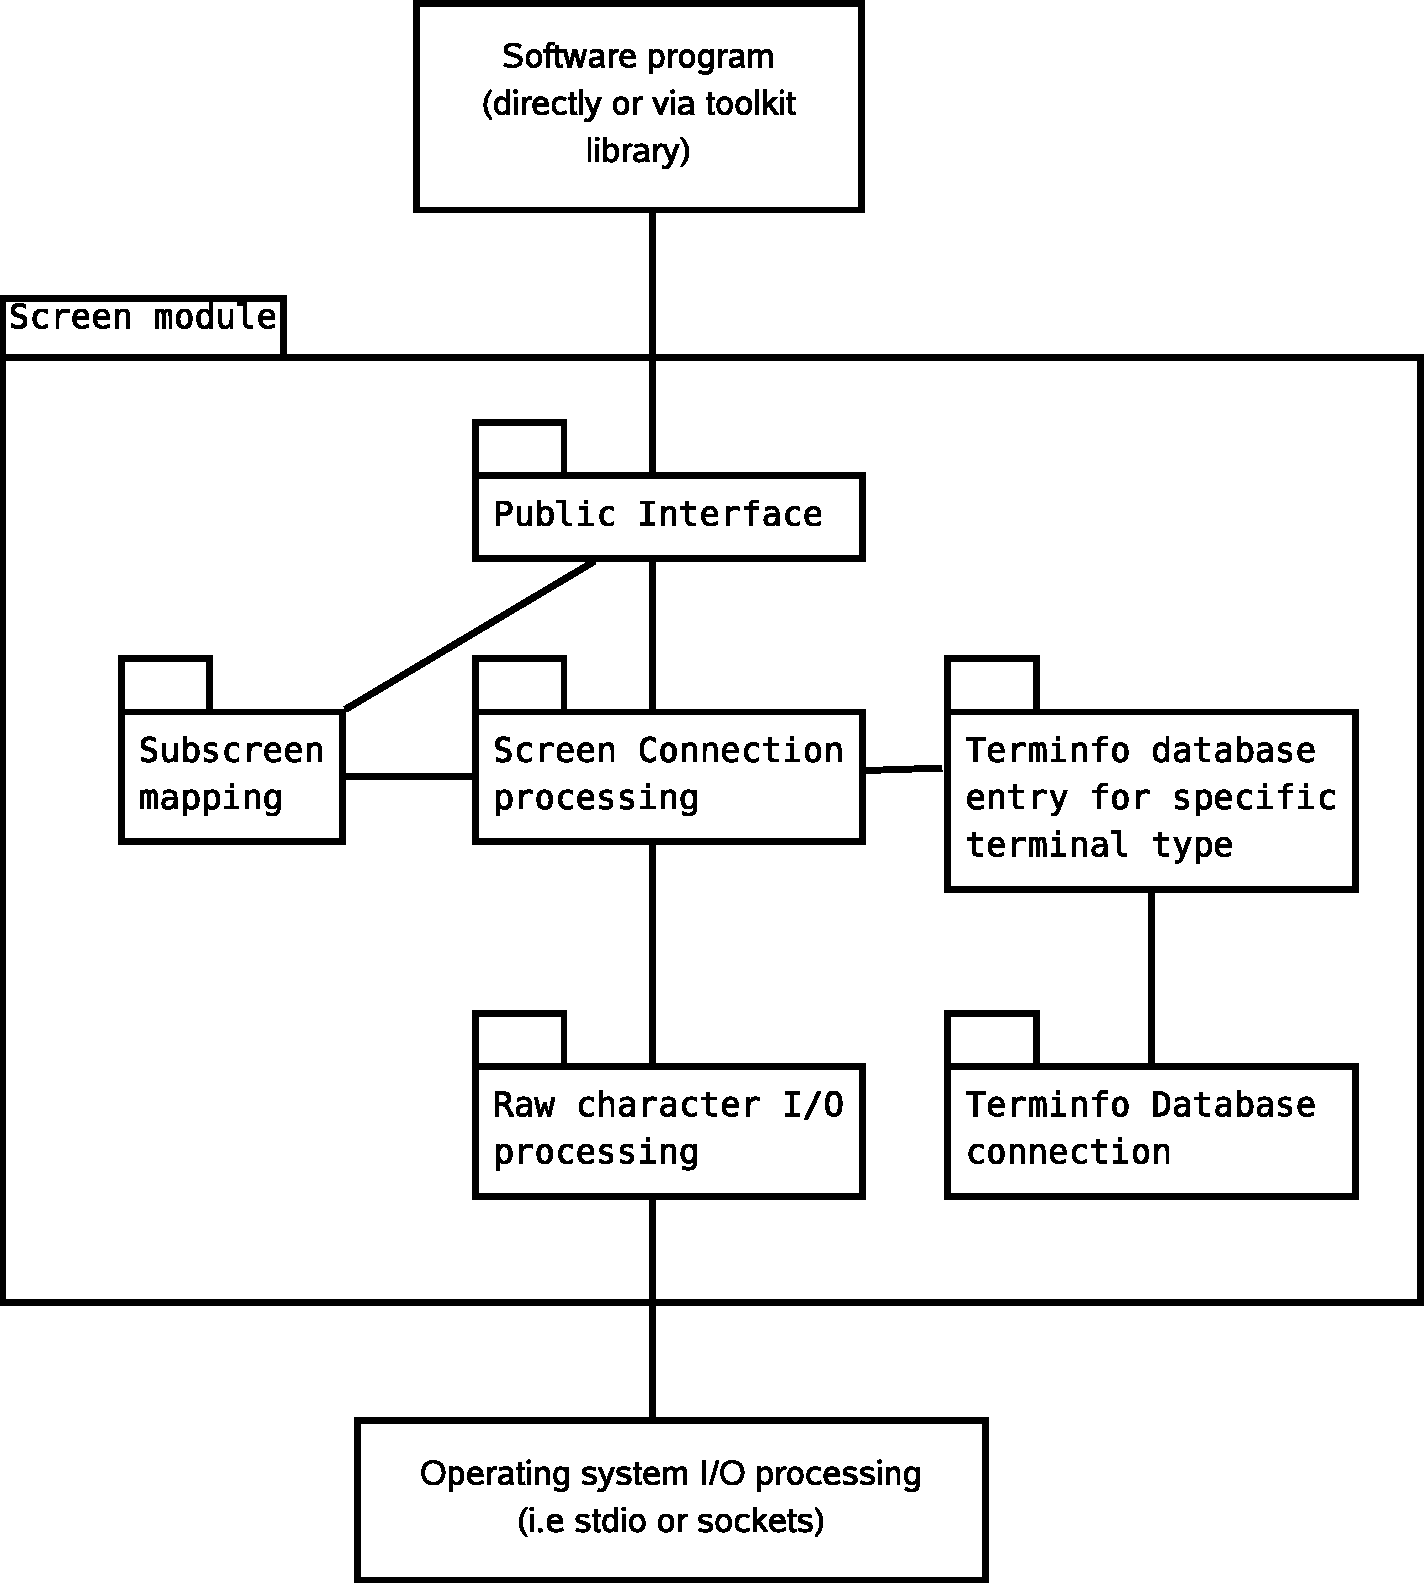
\includegraphics[width=280pt]{graphics/ModuleLayout}
  \end{center}
  \end{figure}
  Each of them is implemented as set of classes with specific
  interfaces between them. Some design principles with brief rationale
  are provided in subsequent sections.


\subsubsection{Thread safety}
  note: ,,module'' symbol in following diagram depicts single instance
  of specific subsystem (functional block):
  \index{thread}
  \advanced

  \begin{figure}[H]
  \begin{center}
  \leavevmode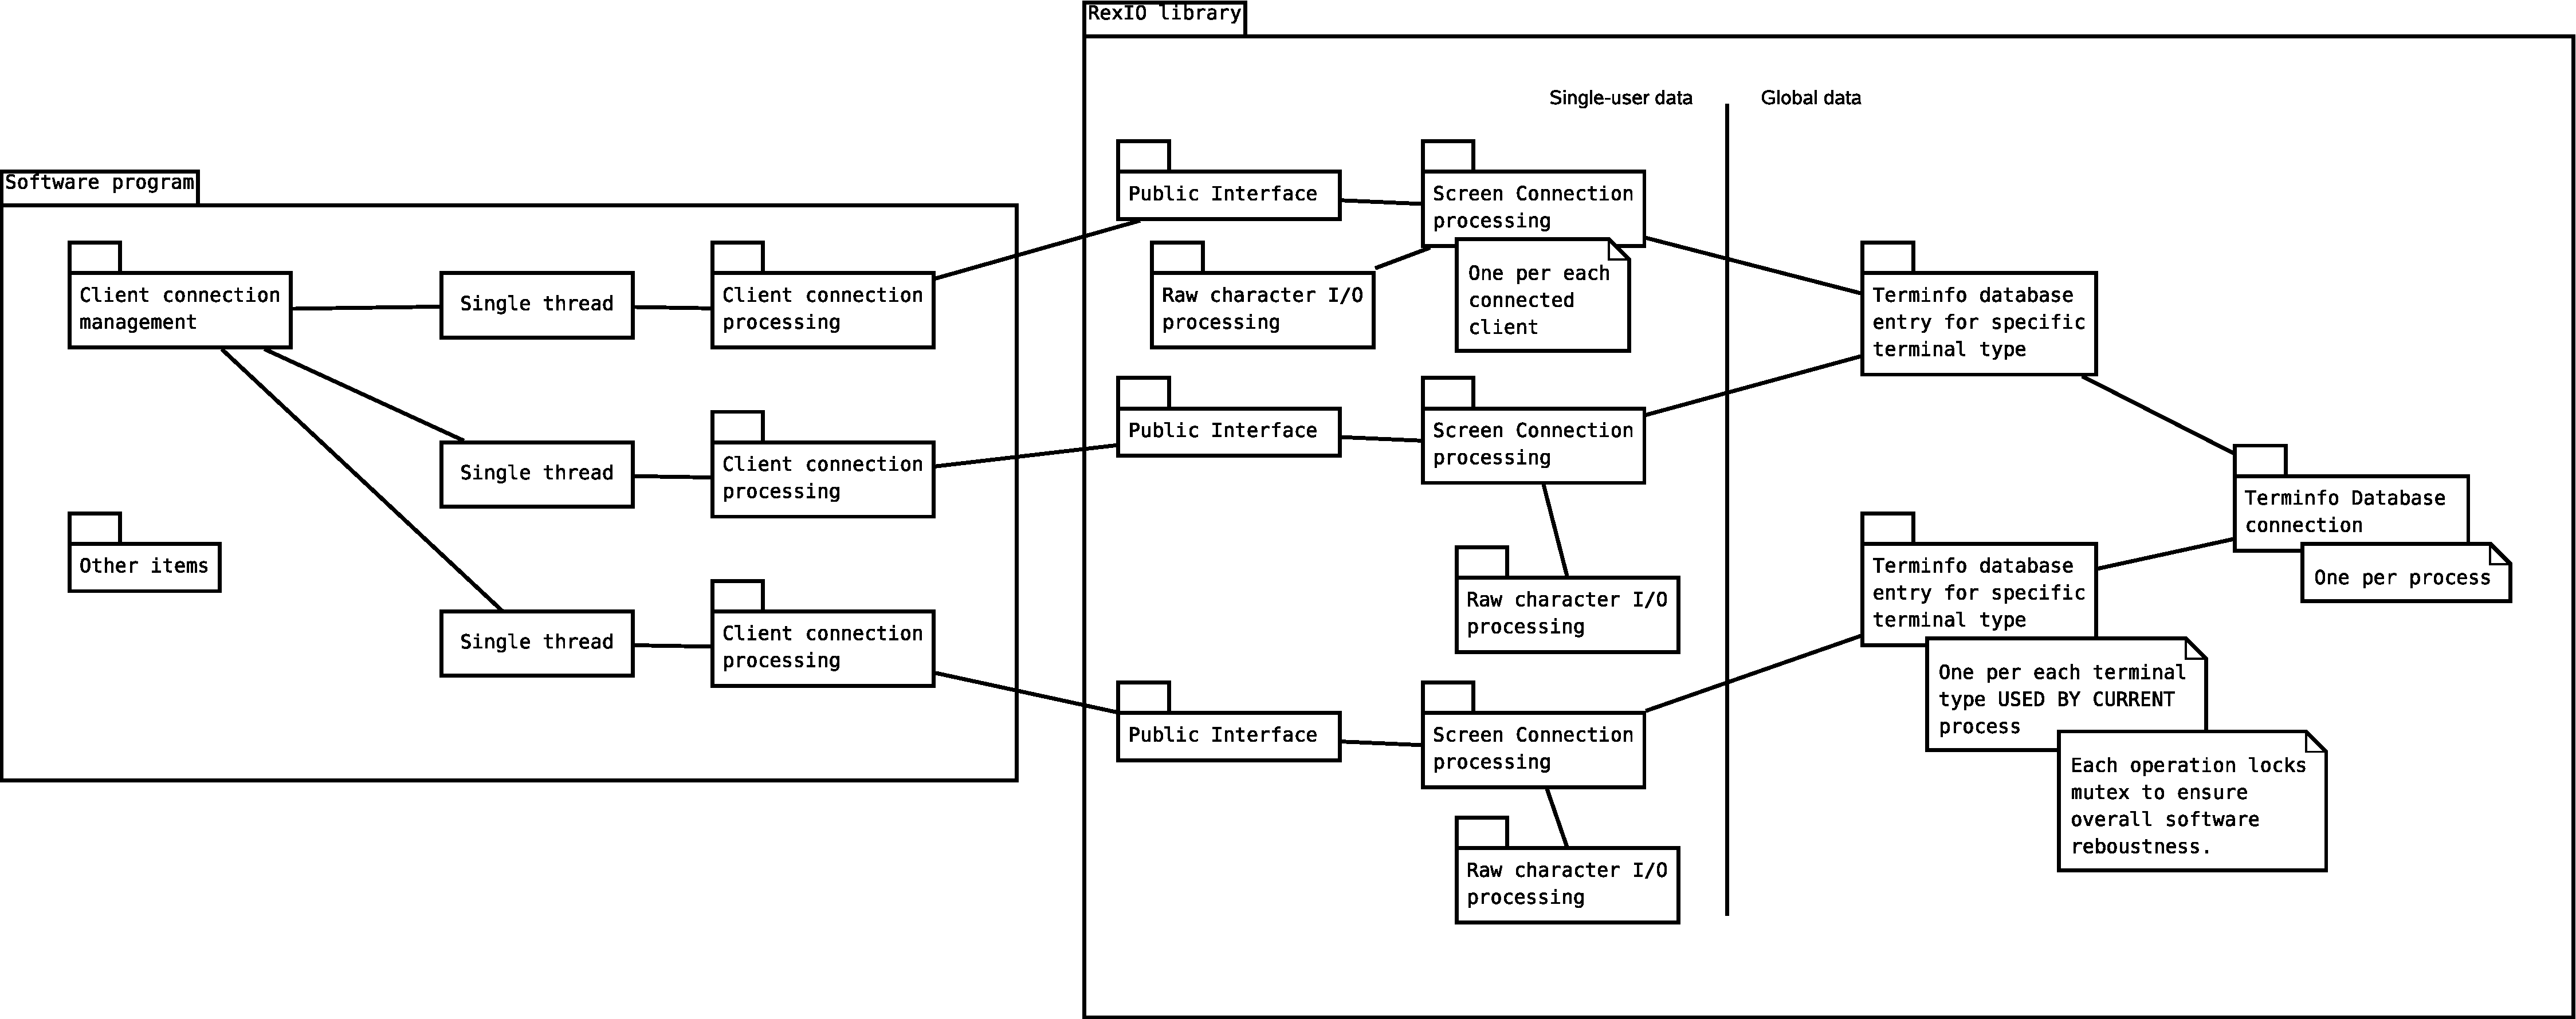
\includegraphics[width=540pt,angle=270]{graphics/MultiThread}
  \end{center}
  \end{figure}
  
  \pagebreak

  Figure on previous page describes typical layout of
  multi-threading-connected features, as well as measures taken to
  obtain stability in threaded programs and ensure their reasonable
  performance.

  As it can be seen, only global data structures are connected to
  TERMINFO database processing, and other items are separated (one per
  connection) to achieve reasonable compromise between versatility and
  efficiency.

  \important
  General guidelines for writing threaded applications using this
  library are as follows:
  
  \begin{itemize}
  \item multiple connections may be created and simultaneously
    processed in multiple threads (guaranteed by library design).
  \item multiple operations at the same moment for SINGLE connection
    are not guaranteed by library design, and therefore special
    measures must be taken while designing software program that uses
    this approach. 
  \end{itemize}
  

\subsubsection{Screen connection processing}
  Screen class generalizes basic screen operations. Support for
  different screen and connection types is implemented through
  inheritance with  multiple polymorphism. RScreen (Real Screen
  Implementation) template generalizes this idea while still allowing
  to take advantage of OOP (Object Oriented Programming).
  \index{subsystems}

  Typical instance of RScreen template looks like this:

  \begin{figure}[H]
  \begin{center}
  \leavevmode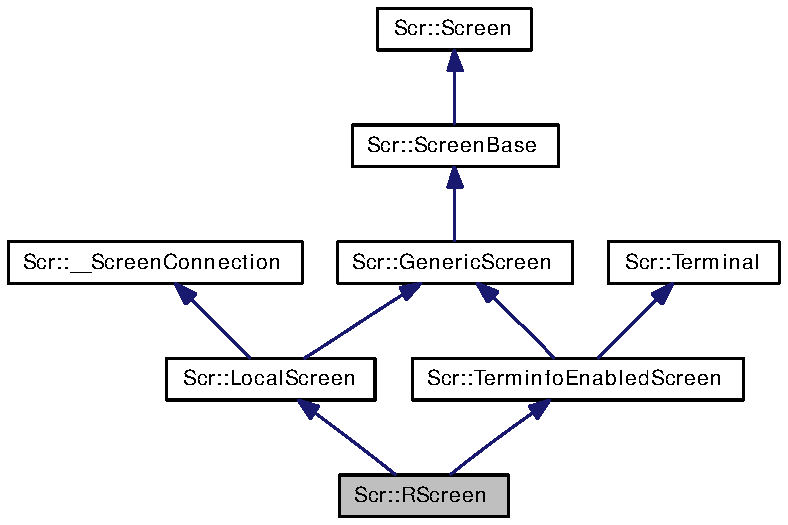
\includegraphics[width=200pt]{graphics/classScr_1_1RScreen__inherit__graph}
  \end{center}
  \end{figure}

  Please note, that fully implementing all this functionality almost
  always involves multitude of object. For example simplified
  collaboration diagram for RScreen implementing local screen that is
  using TERMINFO database looks as follows:

  \begin{figure}[H]
  \begin{center}
  \leavevmode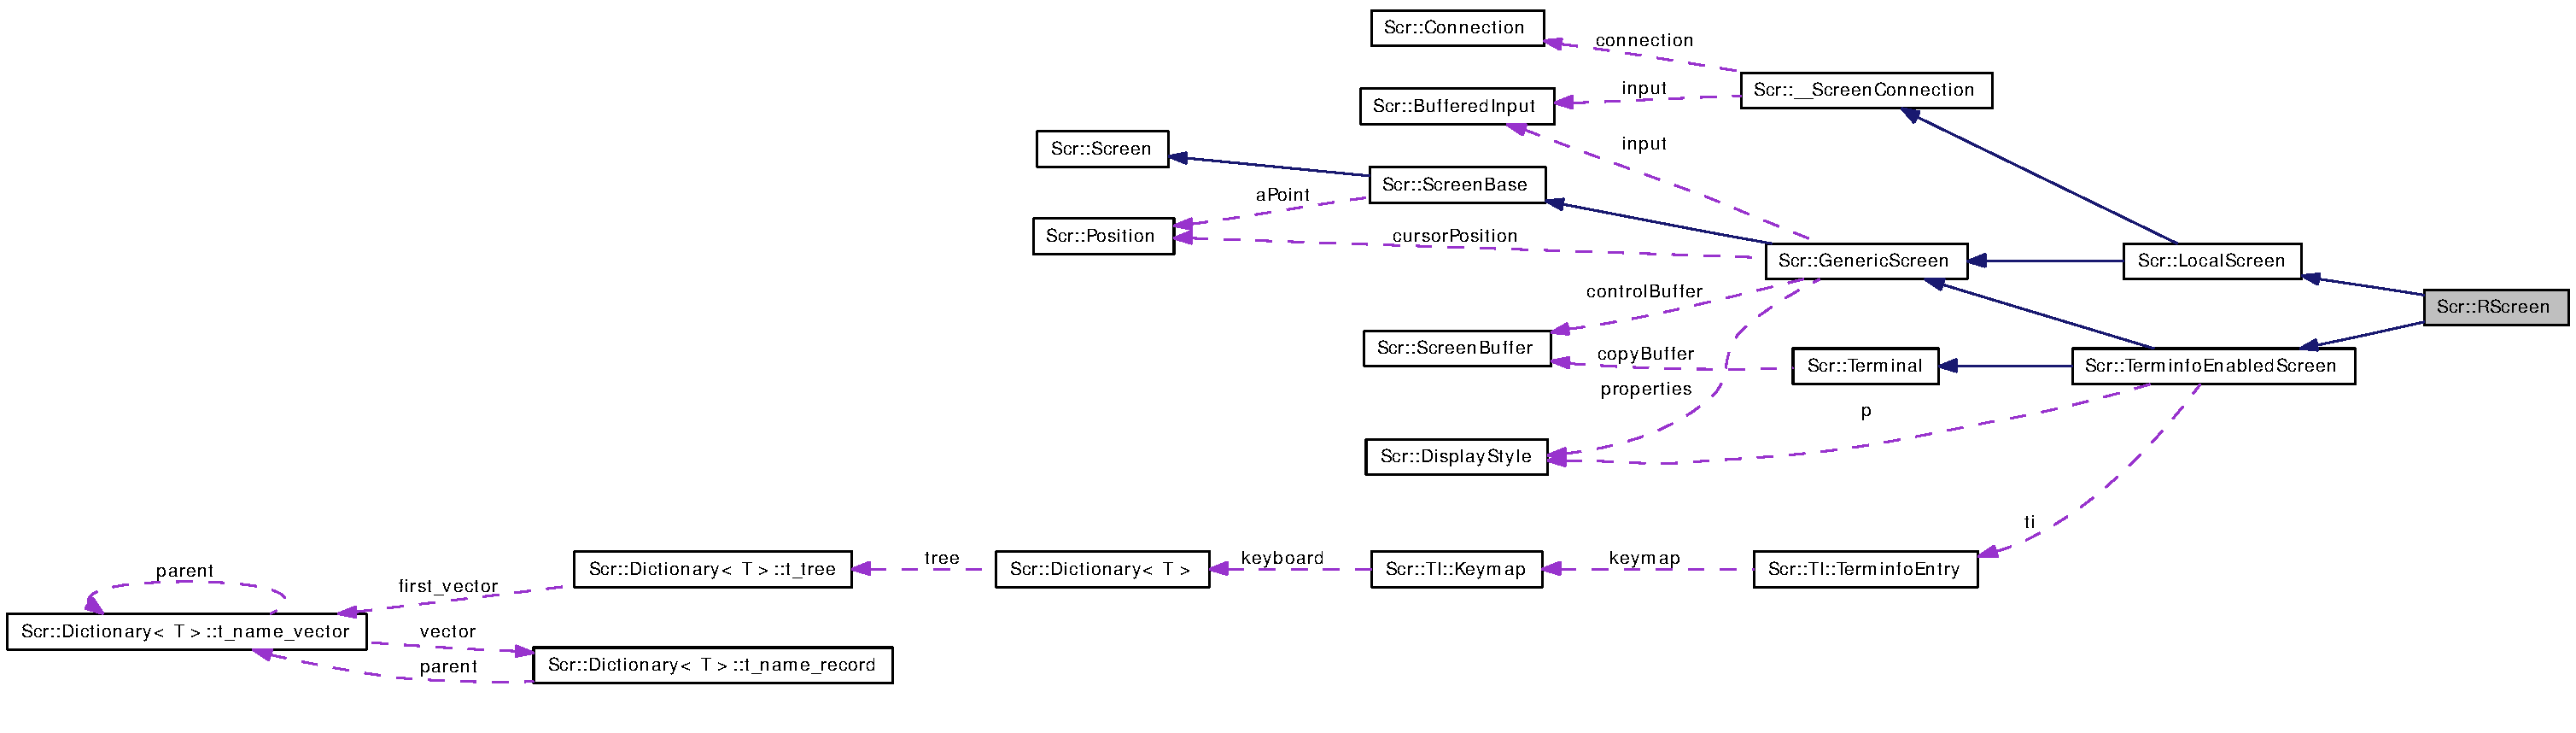
\includegraphics[width=580pt,angle=270,trim=560pt 0 0 0,clip=true]{graphics/classScr_1_1RScreen__coll__graph}
  \end{center}
  \end{figure}

\subsubsection{Sub screen mapping}
  \begin{figure}[H]
  \begin{center}
  \leavevmode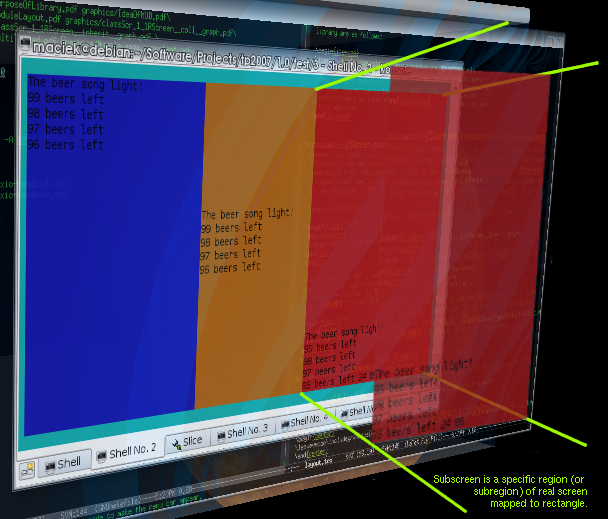
\includegraphics[width=270pt]{graphics/SubscreenMapping}
  \end{center}
  \end{figure}
  \index{subscreen}
  \index{screenshot}
  To fully unite interface and provide efficient way  of designing
  hierarchical display  structures (as user interfaces) concept of
  sub-screen is introduced. Sub-screen is section of screen and is
  itself representative of class screen (inheritance-and-composition
  pattern). 

  \important

  Each basic operation supported by screen is also supported by
  subscreen, as it inherits its interface. Each subscreen operation
  is therefore executed on physical screen with appropriate coordinate
  mapping. Most of these operations affects real screen directly, as
  subscreen doesn't have its own buffer (therefore active point
  coordinates of real screen are not preserved after writing on
  subscreen).

  Please refer to Reference Manual for further details.

\subsubsection{UI Toolkit}
  Scr::Tk namespace contains Widget class that is base to all UI toolkit elements
  Following diagrams demonstrate most of Widget descendents:


  \begin{figure}[H]
  \begin{center}
  \leavevmode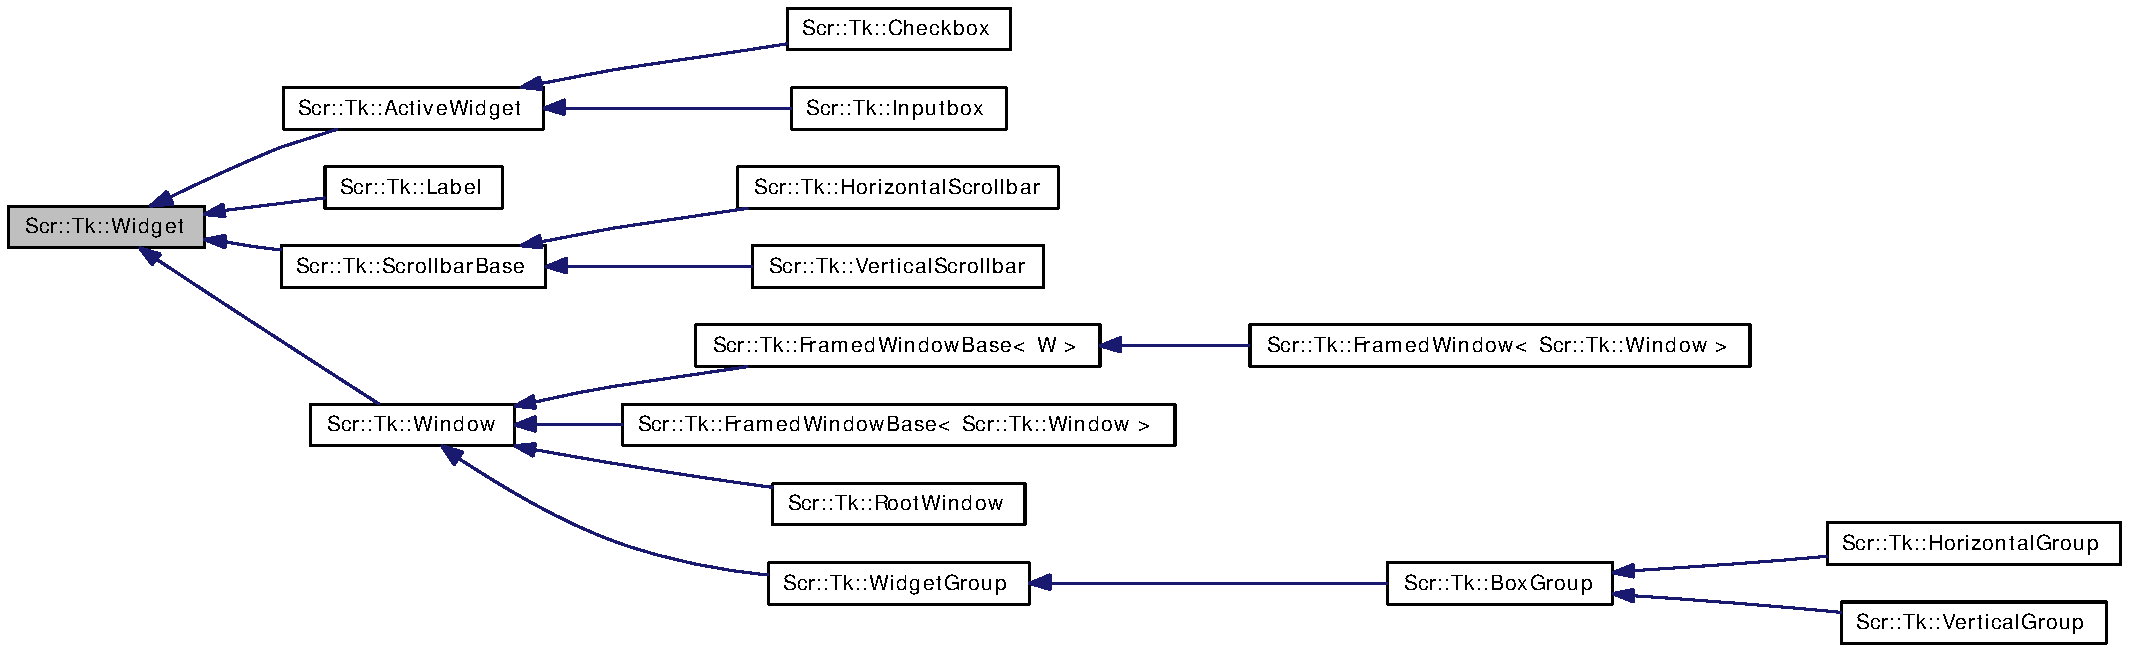
\includegraphics[width=\linewidth,trim=0 0 430pt  0,clip=true]{graphics/classScr_1_1Tk_1_1Widget__inherit__graph}
  \end{center}
  \end{figure}
  \index{toolkit}


  \begin{figure}[H]
  \begin{center}
  \leavevmode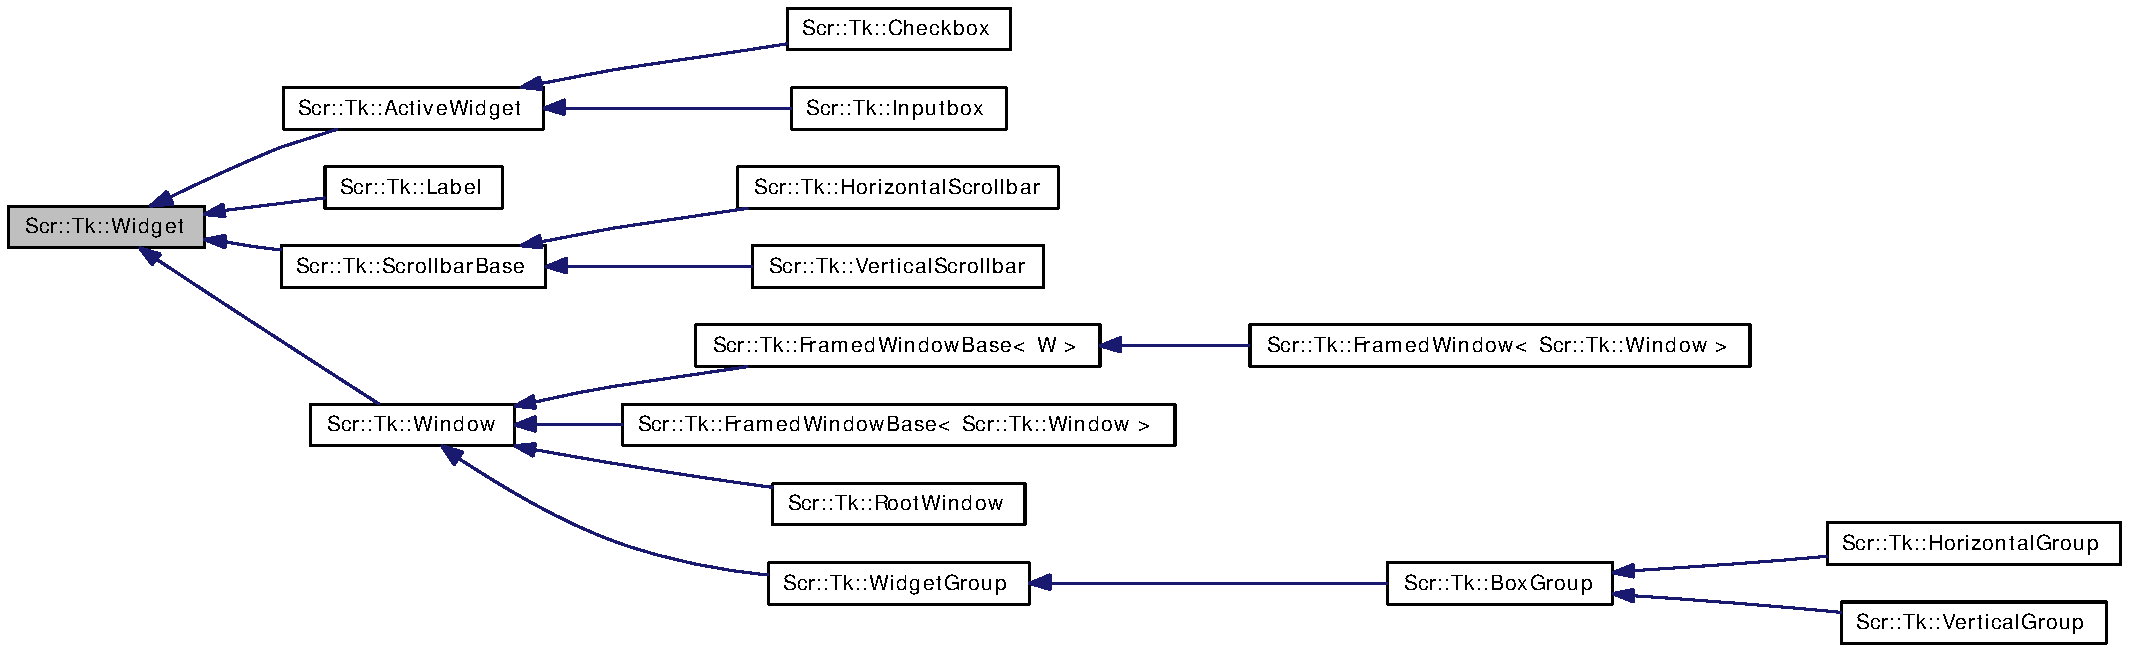
\includegraphics[width=\linewidth,trim=250pt  0  0 150pt ,clip=true]{graphics/classScr_1_1Tk_1_1Widget__inherit__graph}
  \end{center}
  \end{figure}

  Each of them is placed in RootWindow
  
  \begin{figure}[H]
  \begin{center}
  \leavevmode\includegraphics[width=\linewidth]{../latex/classScr_1_1Tk_1_1RootWindow__coll__graph}
  \end{center}
  \end{figure}


% LocalWords:  namespace
